\chapter{A Little Archaeology} 
\label{sec:archaeo}
\lstset{style=6502Style}

Iridis Alpha was distributed on cassette tape by the publisher Hewson Consultants. Normally used
to play audio, cassette tapes were the cheap and ubiquitous medium du jour of the 1980s and a
natural choice for the nascent 8-bit game industry to disribute its wares.

\begin{figure}[H]
  {
    \begin{adjustbox}{width=10cm,center}
      \surface{archaeo/ia-tape.jpg}
    \end{adjustbox}
  }\caption[]{It should be simple getting bytes off this\, right?}
\end{figure}

Playing a cassette tape for a C64 game such as Iridis Alpha on a normal cassette tape player would
be an ear-splitting mistake. Instead of music you would be subjected to a cacophony of mechanical
chirruping. This is the tape attempting to convey to you its long stream of binary data in the only
language available to it: lots of sound waves of varying length.

Without knowing how it's actually done, it's tempting to imagine a variety of possible schemes that
might have been used. For example, one sound wave denoting a '0' and another one denoting a '1'.
The actual method used isn't very far away from such a thing but there is plenty of intricacy
layered on top, particularly in a bid to spend as little time as possible loading data from the
tape.

In order to get something to work with our first step is to somehow convert the contents of the
cassette tape into a binary file so that we can emulate the steps the C64's tape player performed
to read the sounds from the tape and load them into memory as something that could be run as a
computer program.

The earliest and most durable attempt at standardizing this was from Per Hakan Sundell in 1997. He
invented what is now known as the 'tap' format for representing the beeps and bloops encoded on the
tape as a file of bits and bytes. The idea is that each byte in the file represents the length of
a pulse. It is the length of these pulses that will ultimately tell us whether we should interpret
a value of 1 or 0. When we get eights 1s and 0s we have a byte. We get enough bytes, we have a program
we can run!

Someone, somewhere has kindly decoded the contents of the Iridis Alpha cassette tape distribution to
a 'tap' file for us. So we have something to dig into. This is going to be a slightly bonkers journey
into the bowels of decoding a 54kb game file from over 500kb of raw data. Every time you think you
are nearly done there will be yet another convolution to wrap your head around. But at the end of it
we will finally have our binary game file and will be ready to figure out how to decipher it into something
approximating the original assembly langage.

\begin{figure}[H]
  {
    \begin{adjustbox}{width=10cm,center}
      \surface{archaeo/spool.png}
    \end{adjustbox}
  }\caption[]{Simple, right? Here each short-pulse sound is represented by a light grey pixel, each medium-duration pulse by a blue pixel,
and each long pulse by a pink pixel. Roughly speaking, gray is a shorthand for 0 bits and dark pixels for 1 bits.}
\end{figure}

\section{The Madness Begins}

This is what the start of the our \icode{iridis-alpha.tap} file looks like:


\begin{figure}[H]
  {
    \setlength{\tabcolsep}{3.0pt}
    \setlength\cmidrulewidth{\heavyrulewidth} % Make cmidrule = 
    \begin{adjustbox}{width=10cm,center}
      \begin{tikzpicture}
        \draw[step=1.0,gray,thin] (0,0) grid (16,7);
        \fill[gray] (0,6) rectangle ++ (12,1);
        \fill[pink] (12,6) rectangle ++ (1,1);
        \fill[cyan] (13,6) rectangle ++ (3,1);
        \fill[lightred] (0,5) rectangle ++ (3,1);
        \node[matrix of math nodes,anchor=south west,inner sep=0pt,
              nodes={draw,minimum size=1cm,anchor=center},
              column sep=-\pgflinewidth,row sep=-\pgflinewidth,font=\ttfamily]
              {
\icode{43} & \icode{36} & \icode{34} & \icode{2D} & \icode{54} & \icode{41} & \icode{50} & \icode{45} & \icode{2D} & \icode{52} & \icode{41} & \icode{57} & \icode{00} & \icode{00} & \icode{00} & \icode{00}  \\
\icode{5A} & \icode{0A} & \icode{08} & \icode{00} & \icode{00} & \icode{5D} & \icode{32} & \icode{2F} & \icode{30} & \icode{2F} & \icode{2F} & \icode{30} & \icode{30} & \icode{31} & \icode{30} & \icode{31}  \\
\icode{30} & \icode{31} & \icode{31} & \icode{2F} & \icode{31} & \icode{31} & \icode{30} & \icode{31} & \icode{30} & \icode{30} & \icode{31} & \icode{30} & \icode{30} & \icode{30} & \icode{31} & \icode{30}  \\
\icode{31} & \icode{31} & \icode{30} & \icode{31} & \icode{31} & \icode{30} & \icode{31} & \icode{30} & \icode{30} & \icode{31} & \icode{30} & \icode{31} & \icode{31} & \icode{30} & \icode{30} & \icode{30}  \\
\icode{31} & \icode{31} & \icode{31} & \icode{30} & \icode{30} & \icode{31} & \icode{30} & \icode{31} & \icode{31} & \icode{31} & \icode{30} & \icode{30} & \icode{30} & \icode{31} & \icode{31} & \icode{30}  \\
\icode{30} & \icode{30} & \icode{31} & \icode{30} & \icode{31} & \icode{30} & \icode{30} & \icode{30} & \icode{31} & \icode{30} & \icode{31} & \icode{31} & \icode{30} & \icode{30} & \icode{30} & \icode{31}  \\
\icode{31} & \icode{31} & \icode{30} & \icode{30} & \icode{31} & \icode{30} & \icode{32} & \icode{31} & \icode{30} & \icode{31} & \icode{30} & \icode{30} & \icode{32} & \icode{31} & \icode{30} & \icode{30}  \\
						  };

      \end{tikzpicture}
    \end{adjustbox}
  }\caption{The leading material read by the Megasave loader in the run up to retrieving game data. The Pilot Bytes are in red, 
the 'Sync Train' in blue, and the Data Header fields from the grey cell onwards.}
\end{figure}

\begin{figure}[H]
  {
    \setlength{\tabcolsep}{3.0pt}
    \setlength\cmidrulewidth{\heavyrulewidth} % Make cmidrule = 
    \begin{adjustbox}{width=14cm,center}

      \begin{tabular}{rllllllll}
        \toprule
        Field Description & Field Value & Note & \\
        \midrule
TAP Format Header Description & \icode{43 36 34 2D 54 41 50 45 2D 52 41 57}  & 'C64-TAPE-RAW' in ASCII\\
Version & \icode{00} & Version Number 0\\
Reserved & \icode{00 00 00} & Used by format versions > 0\\
File Size & \icode{5A 0A 08} & \$080A05, in decimal: 526,853 bytes long.\\
        \midrule
Start of Data & \makecell{
\icode{00 00 5D 32 2F 30 2F 2F 30 30 31 30 31  } \\
\icode{30 31 31 2F 31 31 30 31 30 30 31 30 30 30 31 30  } \\
\icode{31 31 30 31 31 30 31 30 30 31 30 31 31 30 30 30  } \\
\icode{31 31 31 30 30 31 30 31 31 31 30 30 30 31 31 30  } \\
\icode{30 30 31 30 31 30 30 30 31 30 31 31 30 30 30 31  } \\
\icode{31 31 30 30 31 30 32 31 30 31 30 30 32 31 30 30  } \\
 } & \makecell{
Bytes representing the invdividual \\ pulses/sounds on the tape.  \\
} \\
        \addlinespace
        \bottomrule
      \end{tabular}
    \end{adjustbox}
  }\caption{The meaning of the first batch of data we've read in.}
\end{figure}

After the header information described above, each byte in the \icode{tap} file
represents the pulse length or duration of a single sound emitted by the tape.
A pair of sounds taken together represent a single bit, i.e. a \icode{0} or a
\icode{1}. A medium length sound followed by a short one represents a \icode{1},
a short one followed by a medium one represents a \icode{0}.

The following table shows us whether we should consider a byte on the tape to
represent short, medium, or long
duration sound:

\begin{figure}[H]
  {
    \setlength{\tabcolsep}{3.0pt}
    \setlength\cmidrulewidth{\heavyrulewidth} % Make cmidrule = 
    \begin{adjustbox}{width=7cm,center}

      \begin{tabular}{rllllllll}
        \toprule
        Sound Length & Lower Range & Upper Range & \\
        \midrule
        Short & \icode{\$24}  & \icode{\$36} \\
        Medium & \icode{\$37}  & \icode{\$49} \\
        Long & \icode{\$4A}  & \icode{\$64} \\
        \addlinespace
        \bottomrule
      \end{tabular}

    \end{adjustbox}

  }\caption{Values for short, medium, and long pulses. For example, ny byte value on the \icode{tap} file between \icode{\$24} and
\icode{\$36} would be considered a 'Short' pulse.}
\end{figure}

Remarkably the first 27,000 or so pulses on the Iridis Alpha tape are nothing but short sounds (values between \icode{\$2F} and
\icode{\$31}) so cannot be interpreted as anything. It's not until the 27,157th byte in the tape that we start to encounter real data:

\begin{lstlisting}[caption=Data finally gets started at \icode{56 41} in the first line above.,basicstyle=\tiny]
00006a10: 3031 3031 3156 4144 3130 4231 4243 3130  01011VAD10B1BC10
00006a20: 4231 4131 4244 312f 4057 4032 4231 4231  B1A1BD1/@W@2B1B1
00006a30: 4244 312f 4231 4231 4243 3142 3055 4144  BD1/B1B1BC1B0UAD
00006a40: 3142 3143 3130 4231 4231 4232 4244 3142  1B1C10B1B1B2BD1B
00006a50: 3055 4131 4243 3142 3130 4231 4231 4231  0UA1BC1B10B1B1B1
00006a60: 4244 3130 4056 4143 3230 4143 3130 4231  BD10@VAC20AC10B1
00006a70: 4231 4232 4244 312f 4056 4232 4231 4243  B1B2BD1/@VB2B1BC
00006a80: 3230 4231 4231 4231 4243 3142 2f54 4245  20B1B1B1BC1B/TBE
00006a90: 3141 3130 4231 4231 4230 4230 4243 3030  1A10B1B1B0B0BC00
\end{lstlisting}

The first meaningful twenty bytes therefore are:
\begin{lstlisting}
56 41 44 31 30 42 31 42 43 31 30 42 31 41 31 42 44 31 2F 40
\end{lstlisting}

You get a sense of how wasteful, or ahem redundant, this encoding scheme is when you learn that these twenty pulses are
required to give us a single byte. The table below shows how we interpret them to construct a series of 1s and 0s.

\begin{figure}[H]
  {
    \setlength{\tabcolsep}{3.0pt}
    \setlength\cmidrulewidth{\heavyrulewidth} % Make cmidrule = 
    \begin{adjustbox}{width=9cm,center}

      \begin{tabular}{rllllllll}
        \toprule
        First Byte& Second Byte & First Byte Pulse Length & Second Byte Pulse Length & Meaning & \\
        \midrule
				\icode{\$56} & \icode{\$41}  & Long & Medium & Start of Byte Indicator  \\
				\icode{\$44} & \icode{\$31}  & Medium & Short & \icode{\$01} \\
				\icode{\$30} & \icode{\$42}  & Short & Medium & \icode{\$00} \\
				\icode{\$31} & \icode{\$42}  & Short & Medium & \icode{\$00} \\
				\icode{\$43} & \icode{\$31}  & Medium & Short & \icode{\$01} \\
				\icode{\$30} & \icode{\$42}  & Short & Medium & \icode{\$00} \\
				\icode{\$31} & \icode{\$41}  & Short & Medium & \icode{\$00} \\
				\icode{\$31} & \icode{\$42}  & Short & Medium & \icode{\$00} \\
				\icode{\$44} & \icode{\$31}  & Medium & Short & \icode{\$01} \\
				\icode{\$2F} & \icode{\$40}  & Short & Medium & Parity Bit of \icode{\$00} \\
        \addlinespace
        \bottomrule
      \end{tabular}

    \end{adjustbox}

  }\caption{Interpretation of the first 20 meaningful bytes\, creating a byte. The parity bit at the end is a \icode{\$00}
if there are an odd number of 1s and \icode{\$01} if there are an even number of 1s. \icode{10010001} has an odd number of 1s. }
\end{figure}

We can visualize the twenty bytes as a square sound wave. When reading the tape the C64 would interpret these sound pulses as long, short,
or medium to construct a meaning for the entire sequence.

\begin{figure}[H]
{
	\begin{adjustbox}{width=14cm,center}
	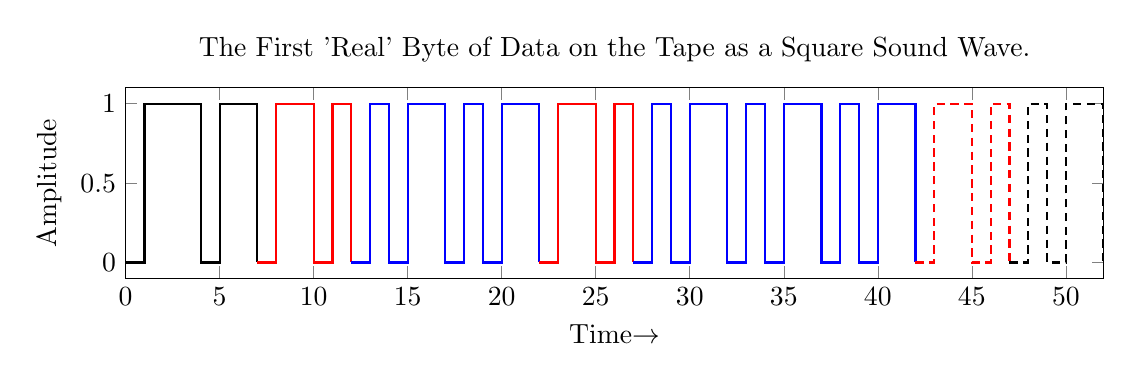
\begin{tikzpicture}
	\begin{axis}[xmin=0,width=14cm,height=4cm,xmax=52,
		title=The First 'Real' Byte of Data on the Tape as a Square Sound Wave.,xlabel={Time$\rightarrow$},ylabel=Amplitude]
			\addplot+[thick,const plot, no marks,black]
			coordinates {(0,0) (1,1) (4,0) (5,1) (7,0) %long medium
			};
	\addplot+[thick,const plot, no marks,red]
		coordinates {
			(7,0) (8,1) (10,0) (11,1) (12,0) % medium short
		};
	\addplot+[thick,const plot, no marks,blue]
		coordinates {
			(12,0) (13,1) (14,0) (15,1) (17,0) % short medium
				(17,0) (18,1) (19,0) (20,1) (22,0) % short medium
		};
	\addplot+[thick,const plot, no marks,red]
		coordinates {
			(22,0) (23,1) (25,0) (26,1) (27,0) % medium short
		};
	\addplot+[thick,const plot, no marks,blue]
		coordinates {
			(27,0) (28,1) (29,0) (30,1) (32,0) % short medium
				(32,0) (33,1) (34,0) (35,1) (37,0) % short medium
				(37,0) (38,1) (39,0) (40,1) (42,0) % short medium
		};
	\addplot+[thick,const plot, no marks,red]
		coordinates {
			(42,0) (43,1) (45,0) (46,1) (47,0) % medium short
		};
	\addplot+[thick,const plot, no marks,black]
		coordinates {
			(47,0) (48,1) (49,0) (50,1) (52,0) % short medium
		};
	\end{axis}
	\end{tikzpicture}
    \end{adjustbox}
}\caption[]{Medium-Short pairs in red represent a '1' bit, Short-Medium pairs in blue represent a '0' bit. So this gives
us '10010001'. The black wave form at the beginning is the 'Start of Byte' indicator\, and the one at the end is a parity bit.}
\end{figure}
Once we've extracted our result of \icode{10010001} from these twenty bytes we now must reverse it. We must do this because
the bits are encoded on the tape with the 'most significant bit' first and we are used to reading binary with the 'least significant bit
first'. In hexadecimal the reversed bit-string of \icode{10001001} is \icode{\$89}.

We have our first byte! It's \icode{89}! 

\section{After Our First Real Byte}
With this precious commodity in hand we now continue reading off bytes in the same manner from the tape. Eventually we encounter
a signal that tells us we've reached the end of the data block, a 'Long-Short' sequence. When this happens we find we've
read 202 bytes in total:

\begin{figure}[H]
  {
    \setlength{\tabcolsep}{3.0pt}
    \setlength\cmidrulewidth{\heavyrulewidth} % Make cmidrule = 
    \begin{adjustbox}{width=10cm,center}
      \begin{tikzpicture}
        \draw[step=1.0,gray,thin] (0,0) grid (16,12);
        \fill[lightred] (0,12) rectangle ++ (9,1);
        \fill[lightblue] (9,12) rectangle ++ (1,1);
        \fill[cyan] (10,12) rectangle ++ (2,1);
        \fill[lightgreen] (12,12) rectangle ++ (2,1);
        \fill[pink] (14,12) rectangle ++ (2,1);
        \fill[pink] (0,11) rectangle ++ (14,1);
        \fill[lightgray] (9,0) rectangle ++ (1,1);
        \node[matrix of math nodes,anchor=south west,inner sep=0pt,
              nodes={draw,minimum size=1cm,anchor=center},
              column sep=-\pgflinewidth,row sep=-\pgflinewidth,font=\ttfamily]
              {
	\icode{89} & \icode{88} & \icode{87} & \icode{86} & \icode{85} & \icode{84} & \icode{83} & \icode{82} & \icode{81} & \icode{03} & \icode{A7} & \icode{02} & \icode{04} & \icode{03} & \icode{49} & \icode{52} \\
	\icode{49} & \icode{44} & \icode{49} & \icode{53} & \icode{00} & \icode{00} & \icode{00} & \icode{00} & \icode{00} & \icode{00} & \icode{00} & \icode{00} & \icode{00} & \icode{00} & \icode{78} & \icode{A9} \\
	\icode{6E} & \icode{8D} & \icode{06} & \icode{DD} & \icode{A2} & \icode{01} & \icode{20} & \icode{D4} & \icode{02} & \icode{26} & \icode{F7} & \icode{A5} & \icode{F7} & \icode{C9} & \icode{63} & \icode{D0} \\
	\icode{F5} & \icode{A0} & \icode{64} & \icode{20} & \icode{E7} & \icode{03} & \icode{C9} & \icode{63} & \icode{F0} & \icode{F9} & \icode{C4} & \icode{F7} & \icode{D0} & \icode{E8} & \icode{20} & \icode{E7} \\
	\icode{03} & \icode{C8} & \icode{D0} & \icode{F6} & \icode{C9} & \icode{00} & \icode{F0} & \icode{D6} & \icode{20} & \icode{E7} & \icode{03} & \icode{99} & \icode{2B} & \icode{00} & \icode{99} & \icode{F9} \\
	\icode{00} & \icode{C8} & \icode{C0} & \icode{0A} & \icode{D0} & \icode{F2} & \icode{A0} & \icode{00} & \icode{84} & \icode{90} & \icode{84} & \icode{02} & \icode{20} & \icode{E7} & \icode{03} & \icode{91} \\
	\icode{F9} & \icode{45} & \icode{02} & \icode{85} & \icode{02} & \icode{E6} & \icode{F9} & \icode{D0} & \icode{02} & \icode{E6} & \icode{FA} & \icode{A5} & \icode{F9} & \icode{C5} & \icode{2D} & \icode{A5} \\
	\icode{FA} & \icode{E5} & \icode{2E} & \icode{90} & \icode{E7} & \icode{20} & \icode{E7} & \icode{03} & \icode{C8} & \icode{84} & \icode{C0} & \icode{58} & \icode{18} & \icode{A9} & \icode{00} & \icode{8D} \\
	\icode{A0} & \icode{02} & \icode{20} & \icode{93} & \icode{FC} & \icode{20} & \icode{53} & \icode{E4} & \icode{A5} & \icode{F7} & \icode{45} & \icode{02} & \icode{05} & \icode{90} & \icode{F0} & \icode{03} \\
	\icode{4C} & \icode{E2} & \icode{FC} & \icode{A5} & \icode{31} & \icode{F0} & \icode{03} & \icode{4C} & \icode{B9} & \icode{02} & \icode{A5} & \icode{32} & \icode{F0} & \icode{03} & \icode{6C} & \icode{2F} \\
	\icode{00} & \icode{20} & \icode{33} & \icode{A5} & \icode{A2} & \icode{03} & \icode{86} & \icode{C6} & \icode{BD} & \icode{F3} & \icode{02} & \icode{9D} & \icode{76} & \icode{02} & \icode{CA} & \icode{D0} \\
	\icode{F7} & \icode{4C} & \icode{E9} & \icode{02} & \icode{A9} & \icode{07} & \icode{85} & \icode{F8} & \icode{20} & \icode{D4} & \icode{02} & \icode{26} & \icode{F7} & \icode{EE} & \icode{20} & \icode{D0} \\
	\icode{C6} & \icode{F8} & \icode{10} & \icode{F4} & \icode{A5} & \icode{F7} & \icode{60} & \icode{00} & \icode{00} & \icode{E4} \\ 
						  };

      \end{tikzpicture}
    \end{adjustbox}
  }\caption{The data we've read in so far. The unshaded section is machine code.}
\end{figure}

Fortunately this data has a meaning. It contains the first part of a machine code program the C64 can execute:

\begin{figure}[H]
  {
    \setlength{\tabcolsep}{3.0pt}
    \setlength\cmidrulewidth{\heavyrulewidth} % Make cmidrule = 
    \begin{adjustbox}{width=12cm,center}

      \begin{tabular}{rllllllll}
        \toprule
        Field Description & Field Value & Note & \\
        \toprule
Countdown & \icode{89 88 87 86 85 84 83 82 81}  & Data Block Header\\
        \midrule
File Type & \icode{03} & 03=PRG, i.e. executable machine code. \\
        \midrule
Load Address & \icode{A7 02} & Address to load to: \icode{\$02A7} \\
End Address & \icode{04 03} & End Address to load to: \icode{\$0304} \\
        \midrule
Filename & \icode{49 52 49 44 49 53 00 00 00 00 00 00 00 00 00 00} & Filename: "IRIDIS"  \\
        \midrule
Machine Code & \makecell{
\icode{78 A9 6E 8D 06 DD A2 01 20 D4 02 26 F7 A5 F7 C9} \\
\icode{63 D0 F5 A0 64 20 E7 03 C9 63 F0 F9 C4 F7 D0 E8} \\
\icode{20 E7 03 C8 D0 F6 C9 00 F0 D6 20 E7 03 99 2B 00} \\
\icode{99 F9 00 C8 C0 0A D0 F2 A0 00 84 90 84 02 20 E7} \\
\icode{03 91 F9 45 02 85 02 E6 F9 D0 02 E6 FA A5 F9 C5} \\
\icode{2D A5 FA E5 2E 90 E7 20 E7 03 C8 84 C0 58 18 A9} \\
\icode{00 8D A0 02 20 93 FC 20 53 E4 A5 F7 45 02 05 90} \\
\icode{F0 03 4C E2 FC A5 31 F0 03 4C B9 02 A5 32 F0 03} \\
\icode{6C 2F 00 20 33 A5 A2 03 86 C6 BD F3 02 9D 76 02} \\
\icode{CA D0 F7 4C E9 02 A9 07 85 F8 20 D4 02 26 F7 EE} \\
\icode{20 D0 C6 F8 10 F4 A5 F7 60 00 00} \\
 } &
\makecell{ This is the machine code of the program to execute. \\
 We will translate this back to assembly so we can understand \\
 what it does later.  \\
} \\
        \midrule
Checksum & \icode{E4} & How is this calculated? \\
        \addlinespace
        \bottomrule
      \end{tabular}

    \end{adjustbox}

  }\caption{The meaning of the data we've read in so far.}
\end{figure}

This small program, once we have loaded the rest of it, is where the fun starts. But before we do that we have lots more
busywork to do. How about reading in all of the above data again from the tape? Yup, that's correct. As we keep
reading the tape we will find that it contains all of the above data a second time, with the slight difference that the 'Data
Block Header' will be \icode{09 08 07 06 05 04 03 02 01} instead of \icode{ 89 88 87 86 85 84 83 82 81}.

We have to read another 23,000 or so more pulses before we get to something new that we're interested in, the second and final part of
the program that we can execute.

When it arrives it looks like this:

\begin{figure}[H]
  {
    \setlength{\tabcolsep}{3.0pt}
    \setlength\cmidrulewidth{\heavyrulewidth} % Make cmidrule = 
    \begin{adjustbox}{width=10cm,center}
      \begin{tikzpicture}
        \draw[step=1.0,gray,thin] (0,0) grid (16,6);
        \fill[lightred] (0,6) rectangle ++ (9,1);
        \fill[lightgray] (6,0) rectangle ++ (1,1);
        \node[matrix of math nodes,anchor=south west,inner sep=0pt,
              nodes={draw,minimum size=1cm,anchor=center},
              column sep=-\pgflinewidth,row sep=-\pgflinewidth,font=\ttfamily]
              {
\icode{89} & \icode{88} & \icode{87} & \icode{86} & \icode{85} & \icode{84} & \icode{83} & \icode{82} & \icode{81} & \icode{A9} & \icode{80} & \icode{05} & \icode{91} & \icode{4C} & \icode{EF} & \icode{F6} \\
\icode{A9} & \icode{A7} & \icode{78} & \icode{8D} & \icode{28} & \icode{03} & \icode{A9} & \icode{02} & \icode{8D} & \icode{29} & \icode{03} & \icode{58} & \icode{A0} & \icode{00} & \icode{84} & \icode{C6} \\
\icode{84} & \icode{C0} & \icode{84} & \icode{02} & \icode{AD} & \icode{11} & \icode{D0} & \icode{29} & \icode{EF} & \icode{8D} & \icode{11} & \icode{D0} & \icode{CA} & \icode{D0} & \icode{FD} & \icode{88} \\
\icode{D0} & \icode{FA} & \icode{78} & \icode{4C} & \icode{51} & \icode{03} & \icode{AD} & \icode{0D} & \icode{DC} & \icode{29} & \icode{10} & \icode{F0} & \icode{F9} & \icode{AD} & \icode{0D} & \icode{DD} \\
\icode{8E} & \icode{07} & \icode{DD} & \icode{4A} & \icode{4A} & \icode{A9} & \icode{19} & \icode{8D} & \icode{0F} & \icode{DD} & \icode{60} & \icode{20} & \icode{8E} & \icode{A6} & \icode{A9} & \icode{00} \\
\icode{A8} & \icode{91} & \icode{7A} & \icode{4C} & \icode{74} & \icode{A4} & \icode{52} & \icode{D5} & \icode{0D} & \icode{00} & \icode{00} & \icode{00} & \icode{00} & \icode{00} & \icode{00} & \icode{00} \\
\icode{00} & \icode{00} & \icode{8B} & \icode{E3} & \icode{AE} & \icode{02} & \icode{53} \\
						  };

      \end{tikzpicture}
    \end{adjustbox}
  }\caption{The data we've read in so far. The unshaded section is machine code.}
\end{figure}

\begin{figure}[H]
  {
    \setlength{\tabcolsep}{3.0pt}
    \setlength\cmidrulewidth{\heavyrulewidth} % Make cmidrule = 
    \begin{adjustbox}{width=12cm,center}

      \begin{tabular}{rllllllll}
        \toprule
        Field Description & Field Value & Note & \\
        \toprule
Countdown & \icode{89 88 87 86 85 84 83 82 81}  & Data Block Header\\
        \midrule
Machine Code & \makecell{
\icode{A9 80 05 91 4C EF F6 A9 A7 78 8D 28 03 A9} \\
\icode{02 8D 29 03 58 A0 00 84 C6 84 C0 84 02 AD } \\
\icode{11 D0 29 EF 8D 11 D0 CA D0 FD 88 D0 FA 78} \\
\icode{4C 51 03 AD 0D DC 29 10 F0 F9 AD 0D DD 8E} \\
\icode{07 DD 4A 4A A9 19 8D 0F DD 60 20 8E A6 A9} \\
\icode{00 A8 91 7A 4C 74 A4 52 D5 0D 00 00 00 00} \\
\icode{00 00 00 00 00 8B E3 AE 02 } \\
 } & This is the rest of  machine code of the program to execute.  \\
        \midrule
Checksum & \icode{53} & How is this calculated? \\
        \addlinespace
        \bottomrule
      \end{tabular}

    \end{adjustbox}

  }\caption{The meaning of the second batch of data we've read in.}
\end{figure}

\begin{figure}[H]
  {
    \begin{adjustbox}{width=10cm,center}
      \surface{archaeo/tap-loader.png}
    \end{adjustbox}
  }\caption[]{The bytes we've read so far from the tape.}
\end{figure}

Would you be surprised to learn that we have to read in this payload a second time from the tape before we're done?
Let's just assume that you're not and let's move swiftly on to wondering what we're supposed to do with 100 or so
bytes of data we've finally managed to read after listening to some 50,000 chirrups and clicks from cassette tape.

The answer is simple. We load the data we've received into RAM and execute it. We load the second chunk of data
we received at address \icode{\$02A7} (this was given in the 'Load Address' field) and the first chunk of data we received directly after it.

What is this program? It seems a bit short to be Iridis Alpha right? What it is is a whole new program for reading the
rest of the data from the tape. That's right: we've read all this data from the tape to get a program for reading data
from the tape. This type of program is called a 'loader', or perhaps in an effort to justify it's existence, a 'turbo loader'.

\section{A Loader for your Loader}
\begin{figure}[H]
  {
    \begin{adjustbox}{width=10cm,center}
      \surface{archaeo/megasave.png}
    \end{adjustbox}
  }\caption[]{MegaSave loader pictured.}
\end{figure}

The idea is that this little program will do a better job of reading data from the tape and more quickly than the C64 can manage
by itself. There is a whole menagerie of these programs that proliferated in the 1980s with exotic names such as Jetload, Easytape,
Audiogenic and so on. Luigi di Fraia maintains a utility called tapclean that does a great job of identifying and emulating
these loaders and thanks to him we have a disassembled version of the loader we've just found on the Iridis Alpha tape. It has the
quintessentially 1980s moniker 'MegaSave' and as you can see in the listing reproduced below is relatively compact.

\lstinputlisting[basicstyle=\tiny,caption=The data we have just loaded\, translated back into assembly language. This is the MegaSave loader.]
{src/archaeo/megasave/loader.asm}

What does MegaSave do that makes it so much faster than the default C64 tape loader? The simple answer is that it cuts corners
and strips away all of the cautious redundancy we observed when loading the loader itself. Instead of reading 20 bytes (or pulses)
from the tape in order to construct a single byte it just needs 8. It does what we naively thought at the beginning might be
the way to read data from the tape: a long pulse is a 0, a short pulse is a 1, you read 8 of them you have the 8 bits for your
byte.

 
	
This simplicity is risky. With no repetition of data blocks, no parity check on each individual byte, and no delimiters between
bytes, the loader is vulnerable to corruption of the tape itself or any hardware flakiness in the cassette reader. The fact
that it generally works is simply due to a lack of conservatism paying off in practice. In addition, the MegaSave loader isn't
totally bereft of precautions. There is a slightly elaborate dance it goes through to gain some assurance that the tape
medium is going to yield a reliable string of bytes.

The first thing it does is look for a sentinel value of \icode{\$63}. 

\begin{figure}[H]
{
	\begin{adjustbox}{width=14cm,center}
	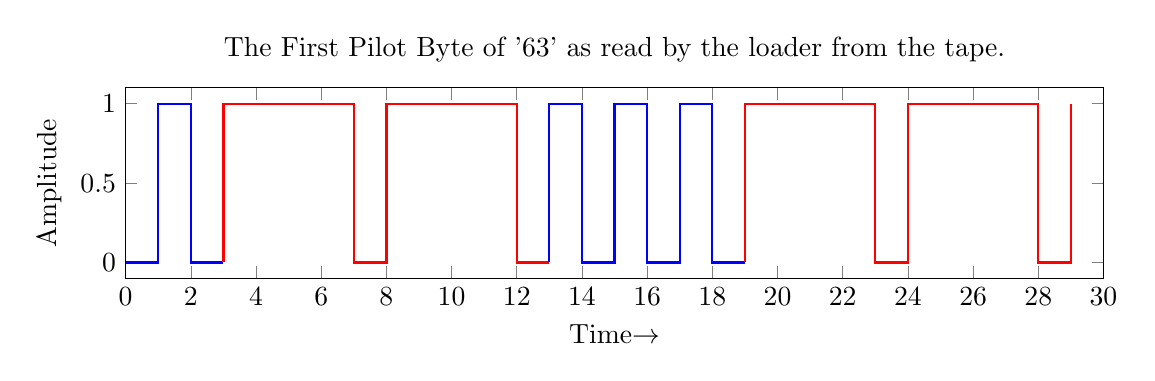
\begin{tikzpicture}
	\begin{axis}[xmin=0,width=14cm,height=4cm,xmax=30,
		title=The First Pilot Byte of '63' as read by the loader from the tape.,xlabel={Time$\rightarrow$},ylabel=Amplitude]
			\addplot+[thick,const plot, no marks,blue]
			coordinates {(0,0) (1,1) (2,0) (3,0) %short
			};
			\addplot+[thick,const plot, no marks,red]
			coordinates {(3,0) (3,1) (6,1) (7,0) (8,1) %long
			(8,1) (11,1) (12,0) (13,0) %long
			};
			\addplot+[thick,const plot, no marks,blue]
			coordinates {(13,0) (13,1) (14,0) (15,1) %short
			(15,1) (16,0) (17,1) %short
			(17,1) (18,1) (18,0) (19,0)  %short
			};
			\addplot+[thick,const plot, no marks,red]
			coordinates {(19,0) (19,1) (22,1) (23,0) (24,1) %long
			(24,1) (27,1) (28,0) (29,1) %long
			};
	\end{axis}
	\end{tikzpicture}
	\end{adjustbox}
}\caption[]{Long square waves in red represent pulses giving a '1' bit, Short square waves in blue represent a '0' bit. So this gives
	us '01100011'\, i.e. \icode{\$63}. Unlike the default tape loader, MegaSave expects the 'most significant bit first' - which is the
natural way of representing bits on paper\, so we don't need to reverse the bits to 'make sense' of them.}.
	\end{figure}

There is an inordinately long string of these, followed by an ascending sequence of byte values from \icode{\$63} to \icode{\$FF}.
This sequence has the catchy name of a 'Sync Train':

\lstdefinestyle{megasave}{
  emptylines=1,
  basicstyle=\small\ttfamily\color{black},
  moredelim=**[is][\color{red}]{@}{@},
  moredelim=**[is][\color{blue}]{~}{~},
}

\begin{figure}[H]
  {
    \setlength{\tabcolsep}{3.0pt}
    \setlength\cmidrulewidth{\heavyrulewidth} % Make cmidrule = 
    \begin{adjustbox}{width=10cm,center}
      \begin{tikzpicture}
        \draw[step=1.0,gray,thin] (0,0) grid (17,19);
        \fill[lightred] (0,19) rectangle ++ (17,1);
        \fill[lightred] (0,18) rectangle ++ (17,1);
        \fill[lightred] (0,17) rectangle ++ (17,1);
        \fill[lightred] (0,16) rectangle ++ (17,1);
        \fill[lightred] (0,15) rectangle ++ (17,1);
        \fill[lightred] (0,14) rectangle ++ (17,1);
        \fill[lightred] (0,13) rectangle ++ (17,1);
        \fill[lightred] (0,12) rectangle ++ (17,1);
        \fill[lightred] (0,11) rectangle ++ (17,1);
        \fill[lightred] (0,10) rectangle ++ (5,1);
        \fill[lightblue] (5,10) rectangle ++ (12,1);
        \fill[lightblue] (0,9) rectangle ++ (17,1);
        \fill[lightblue] (0,8) rectangle ++ (17,1);
        \fill[lightblue] (0,7) rectangle ++ (17,1);
        \fill[lightblue] (0,6) rectangle ++ (17,1);
        \fill[lightblue] (0,5) rectangle ++ (17,1);
        \fill[lightblue] (0,4) rectangle ++ (17,1);
        \fill[lightblue] (0,3) rectangle ++ (17,1);
        \fill[lightblue] (0,2) rectangle ++ (17,1);
        \fill[lightblue] (0,1) rectangle ++ (9,1);
        \fill[lightgray] (9,1) rectangle ++ (1,1);
        \fill[lightgreen] (10,1) rectangle ++ (2,1);
        \fill[yellow] (12,1) rectangle ++ (2,1);
        \fill[cyan] (14,1) rectangle ++ (2,1);
        \fill[pink] (16,1) rectangle ++ (1,1);
        \fill[violet] (0,0) rectangle ++ (1,1);
        \node[matrix of math nodes,anchor=south west,inner sep=0pt,
              nodes={draw,minimum size=1cm,anchor=center},
              column sep=-\pgflinewidth,row sep=-\pgflinewidth,font=\ttfamily]
              {
\icode{63} & \icode{63} & \icode{63} & \icode{63} & \icode{63} & \icode{63} & \icode{63} & \icode{63} & \icode{63} & \icode{63} & \icode{63} & \icode{63} & \icode{63} & \icode{63} & \icode{63} & \icode{63} & \icode{63} \\
\icode{63} & \icode{63} & \icode{63} & \icode{63} & \icode{63} & \icode{63} & \icode{63} & \icode{63} & \icode{63} & \icode{63} & \icode{63} & \icode{63} & \icode{63} & \icode{63} & \icode{63} & \icode{63} & \icode{63} \\
\icode{63} & \icode{63} & \icode{63} & \icode{63} & \icode{63} & \icode{63} & \icode{63} & \icode{63} & \icode{63} & \icode{63} & \icode{63} & \icode{63} & \icode{63} & \icode{63} & \icode{63} & \icode{63} & \icode{63} \\
\icode{63} & \icode{63} & \icode{63} & \icode{63} & \icode{63} & \icode{63} & \icode{63} & \icode{63} & \icode{63} & \icode{63} & \icode{63} & \icode{63} & \icode{63} & \icode{63} & \icode{63} & \icode{63} & \icode{63} \\
\icode{63} & \icode{63} & \icode{63} & \icode{63} & \icode{63} & \icode{63} & \icode{63} & \icode{63} & \icode{63} & \icode{63} & \icode{63} & \icode{63} & \icode{63} & \icode{63} & \icode{63} & \icode{63} & \icode{63} \\
\icode{63} & \icode{63} & \icode{63} & \icode{63} & \icode{63} & \icode{63} & \icode{63} & \icode{63} & \icode{63} & \icode{63} & \icode{63} & \icode{63} & \icode{63} & \icode{63} & \icode{63} & \icode{63} & \icode{63} \\
\icode{63} & \icode{63} & \icode{63} & \icode{63} & \icode{63} & \icode{63} & \icode{63} & \icode{63} & \icode{63} & \icode{63} & \icode{63} & \icode{63} & \icode{63} & \icode{63} & \icode{63} & \icode{63} & \icode{63} \\
\icode{63} & \icode{63} & \icode{63} & \icode{63} & \icode{63} & \icode{63} & \icode{63} & \icode{63} & \icode{63} & \icode{63} & \icode{63} & \icode{63} & \icode{63} & \icode{63} & \icode{63} & \icode{63} & \icode{63} \\
\icode{63} & \icode{63} & \icode{63} & \icode{63} & \icode{63} & \icode{63} & \icode{63} & \icode{63} & \icode{63} & \icode{63} & \icode{63} & \icode{63} & \icode{63} & \icode{63} & \icode{63} & \icode{63} & \icode{63} \\
\icode{63} & \icode{63} & \icode{63} & \icode{63} & \icode{63} & \icode{64} & \icode{64} & \icode{65} & \icode{66} & \icode{67} & \icode{68} & \icode{69} & \icode{6A} & \icode{6B} & \icode{6C} & \icode{6D} & \icode{6E} \\
\icode{6F} & \icode{70} & \icode{71} & \icode{72} & \icode{73} & \icode{74} & \icode{75} & \icode{76} & \icode{77} & \icode{78} & \icode{79} & \icode{7A} & \icode{7B} & \icode{7C} & \icode{7D} & \icode{7E} & \icode{7F} \\
\icode{80} & \icode{81} & \icode{82} & \icode{83} & \icode{84} & \icode{85} & \icode{86} & \icode{87} & \icode{88} & \icode{89} & \icode{8A} & \icode{8B} & \icode{8C} & \icode{8D} & \icode{8E} & \icode{8F} & \icode{90} \\
\icode{91} & \icode{92} & \icode{93} & \icode{94} & \icode{95} & \icode{96} & \icode{97} & \icode{98} & \icode{99} & \icode{9A} & \icode{9B} & \icode{9C} & \icode{9D} & \icode{9E} & \icode{9F} & \icode{A0} & \icode{A1} \\
\icode{A2} & \icode{A3} & \icode{A4} & \icode{A5} & \icode{A6} & \icode{A7} & \icode{A8} & \icode{A9} & \icode{AA} & \icode{AB} & \icode{AC} & \icode{AD} & \icode{AE} & \icode{AF} & \icode{B0} & \icode{B1} & \icode{B2} \\
\icode{B3} & \icode{B4} & \icode{B5} & \icode{B6} & \icode{B7} & \icode{B8} & \icode{B9} & \icode{BA} & \icode{BB} & \icode{BC} & \icode{BD} & \icode{BE} & \icode{BF} & \icode{C0} & \icode{C1} & \icode{C2} & \icode{C3} \\
\icode{C4} & \icode{C5} & \icode{C6} & \icode{C7} & \icode{C8} & \icode{C9} & \icode{CA} & \icode{CB} & \icode{CC} & \icode{CD} & \icode{CE} & \icode{CF} & \icode{D0} & \icode{D1} & \icode{D2} & \icode{D3} & \icode{D4} \\
\icode{D5} & \icode{D6} & \icode{D7} & \icode{D8} & \icode{D9} & \icode{DA} & \icode{DB} & \icode{DC} & \icode{DD} & \icode{DE} & \icode{DF} & \icode{E0} & \icode{E1} & \icode{E2} & \icode{E3} & \icode{E4} & \icode{E5} \\
\icode{E6} & \icode{E7} & \icode{E8} & \icode{E9} & \icode{EA} & \icode{EB} & \icode{EC} & \icode{ED} & \icode{EE} & \icode{EF} & \icode{F0} & \icode{F1} & \icode{F2} & \icode{F3} & \icode{F4} & \icode{F5} & \icode{F6} \\
\icode{F7} & \icode{F8} & \icode{F9} & \icode{FA} & \icode{FB} & \icode{FC} & \icode{FD} & \icode{FE} & \icode{FF} & \icode{01} & \icode{00} & \icode{08} & \icode{FF} & \icode{BF} & \icode{00} & \icode{00} & \icode{01} \\
\icode{02} & \icode{CA} & \icode{00} \\
						  };

      \end{tikzpicture}
    \end{adjustbox}
  }\caption{The leading material read by the Megasave loader in the run up to retrieving game data. The Pilot Bytes are in red, 
the 'Sync Train' in blue, and the Data Header fields from the grey cell onwards.}
\end{figure}

The bytes after the blue cells above are our first bit of raw meat in a while. Here's what they mean:

\begin{figure}[H]
  {
    \setlength{\tabcolsep}{3.0pt}
    \setlength\cmidrulewidth{\heavyrulewidth} % Make cmidrule = 
    \begin{adjustbox}{width=12cm,center}

      \begin{tabular}{rllllllll}
        \toprule
        Field Description & Field Value & Note & \\
        \toprule
Header Sentinel & \icode{01}  & Indicates the start of the header, expected to be non zero.\\
        \midrule
Load Address & \icode{00 08} & Address to load to: \icode{\$0800} \\
        \midrule
End Address & \icode{FF BF} & End Address to load to: \icode{\$BFFF} \\
        \midrule
Execution Address & \icode{00 00} & Filename: "IRIDIS"  \\
        \midrule
Next Action Indicator & \icode{01} & Resume loading data when done or execute the loaded data.\\
        \midrule
Execution Type & \icode{02} & How to execute the code.\\
        \midrule
        \addlinespace
        \bottomrule
      \end{tabular}

    \end{adjustbox}

  }\caption{The meaning of the Data Header values read in by MegaSave.}
\end{figure}

What the loader can garner from this is that the data that follows should be read in and stored at \icode{\$0800}
and that rather than execute it straight away it should then resume loading more data from the tape.

The entire game is stored across four separate chunks on the tape. Once it has loaded this first one, the loader
reads in the next three chunks.

\begin{figure}[H]
  {
    \begin{adjustbox}{width=10cm,center}
      \surface{archaeo/tap-full.png}
    \end{adjustbox}
  }\caption[]{All the data that has been read from the tape. The four chunks of game data are in green\, the third is only a sliver. The
relative sizes of the red data (the MegaSave loader which is only actually 200 or so bytes long) and the green data (representing over
50,000 bytes of game data) illustrates how efficient the MegaSave loader's storage is by comparison with the default.}
\end{figure}

\begin{figure}[H]
  {
    \begin{adjustbox}{width=10cm,center}
      \surface{archaeo/spool-sections.png}
    \end{adjustbox}
  }\caption[]{Our image of the spool from the start of this chapter but this time with each section colored in as described in the previous image.}
\end{figure}

When it has completed it has loaded the following to RAM:

\begin{figure}[H]
  {
    \setlength{\tabcolsep}{3.0pt}
    \setlength\cmidrulewidth{\heavyrulewidth} % Make cmidrule = 
    \begin{adjustbox}{width=5cm,center}

      \begin{tabular}{rllllllll}
        \toprule
        Start Address & End Address & Note & \\
        \toprule
\icode{0800} & \icode{BFFE}  & .\\
\icode{BF00} & \icode{BFFF}  & .\\
\icode{C000} & \icode{CFFE}  & .\\
\icode{E000} & \icode{F7FF}  & .\\
        \addlinespace
        \bottomrule
      \end{tabular}

    \end{adjustbox}

  }\caption{The four chunks of game data.}
\end{figure}

\begin{figure}[H]
  {
    \begin{adjustbox}{width=14cm,center}
      \surface{archaeo/layout.png}
    \end{adjustbox}
  }\caption[]{Where the different parts of the game end up in memory.}
\end{figure}

\section{Putting an End to the Madness}

With all the data read in you might wonder how the loader knows what to do next (i.e. to run the game) and how it
will know where to start running it from. The answer is given in the \icode{Header Data} for the final chunk of data:

\begin{figure}[H]
  {
    \setlength{\tabcolsep}{3.0pt}
    \setlength\cmidrulewidth{\heavyrulewidth} % Make cmidrule = 
    \begin{adjustbox}{width=12cm,center}

      \begin{tabular}{rllllllll}
        \toprule
        Field Description & Field Value & Note & \\
        \toprule
Header Sentinel & \icode{01}  & Indicates the start of the header, expected to be non zero.\\
        \midrule
Load Address & \icode{00 E0} & Address to load to: \icode{\$E000} \\
        \midrule
End Address & \icode{00 F8} & End Address to load to: \icode{\$F800} \\
        \midrule
Execution Address & \icode{10 08} & Address to start execution at: \icode{\$0810}. \\
        \midrule
Next Action Indicator & \icode{00} & 00 means start executing code, don't read any more data.\\
        \midrule
Execution Type & \icode{02} & How to execute the code: 01 means used the address given in 'Execution Address'.\\
        \midrule
        \addlinespace
        \bottomrule
      \end{tabular}

    \end{adjustbox}

  }\caption{The meaning of the Data Header values in the final chunk of data read in by MegaSave.}
\end{figure}

So according to the header data, the loader should stop reading data now and start executing what has already
been loaded, and it should start doing this at address \icode{\$0810}.

\begin{lstlisting}[caption=The first piece of code that is executed in Iridis Alpha.]
*=$0810
StartExecution
        SEI
        ; Tell the C64 to execute the code at MainControlLoop
        ; the next time an interrupt happens.
        LDA #>MainControlLoop
        STA $0319    ;NMI
        LDA #<MainControlLoop
        STA $0318    ;NMI

        ; Turn off the tape deck.
        LDA #$10
        STA $DD04    ;CIA2: Timer A: Low-Byte
        LDA #$00
        STA $DD05    ;CIA2: Timer A: High-Byte
        LDA #$7F
        STA $DD0D    ;CIA2: CIA Interrupt Control Register
        LDA #$81
        STA $DD0D    ;CIA2: CIA Interrupt Control Register
        LDA #$19
        STA $DD0E    ;CIA2: CIA Control Register A
        CLI
LoopUntilExexcutes
        JMP LoopUntilExexcutes
\end{lstlisting}

This routine does two things: it turns off the tape deck and tells the C64 to execute the code at a different
location (\icode{MainControlLoop}) the next time it wakes up and wonders what to do. This will be in a few
microseconds time. When it starts executing \icode{MainControlLoop}, Iridis Alpha will get underway.

 
\begin{figure}[H]
  {
    \begin{adjustbox}{width=10cm,center}
      \surface{archaeo/ia-title.png}
    \end{adjustbox}
  }\caption[]{A \icode{prg} is born.}
\end{figure}


